%% The following is a directive for TeXShop to indicate the main file
%%!TEX root = main.tex

% ===========================================================================================
\chapter{\textbf{Attacks description and detection}}
\label{ch:Attacks}

In this chapter, the attacks that were emulated on each test-bed are discussed. The attacks that are discussed here are  targeted attacks, which means that they specifically target physical properties of the two \ac{CPS} platforms. Note, that the attacks designed for both the test-beds are intentionally stealthy, i.e. it is expected that the attacker wants to remain undetected while introducing some malicious content to accomplish its goal. Also, attack trees are used for designing attacks on the test-beds. These attack trees are based on prior attacks on very similar systems, thus making them realistic and appropriate for testing \ac{CORGIDS}.


\section{Attacks on \ac{UAV}}

\begin{figure}[ht]
    \centering
    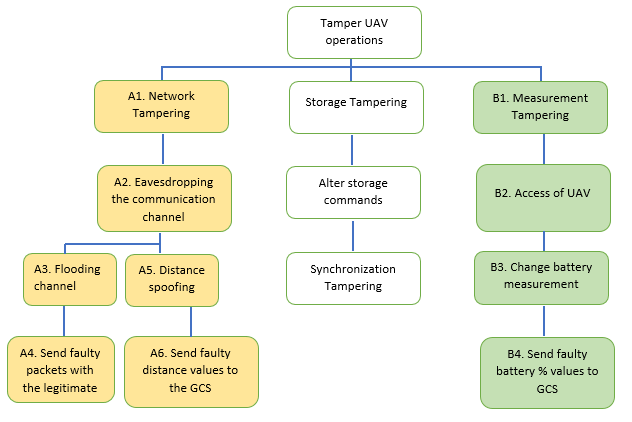
\includegraphics[scale=0.75,keepaspectratio = true]{Graphics/AttackTreeUAVNew.png}
    \caption{Attack tree for UAV}
    \label{fig:attackTreeUAV}
\end{figure}
As discussed above, an \ac{UAV} regularly transmits flight data to the \ac{GCS}, so that it can be tracked throughout its flight. The \ac{GCS} based on the flight data received interprets if the \ac{UAV} is following the instructed guidelines or has drifted from it. An attack tree for faulty \ac{UAV} operations (shown in Figure~\ref{fig:attackTreeUAV}) was formulated, based on attacks introduced in previous work~\cite{javaid2012cyber, mitchell2012specification}. There are three branches in this tree, namely, i) Network Tampering; ii) Storage Tampering; and iii) Measurement Tampering. Two out of the three branches were used to develop attacks which are discussed below.

\begin{itemize}
\item {\bf Battery Tampering Attack (Block B1-B4)}: This attack occurs when an attacker is able to tamper with the control logic of the \ac{UAV} by hacking it. By changing the control logic, the attacker can change the decisions that are made based on the input physical properties from the sensors. Obtaining the access of the \ac{UAV} is not an unreasonable condition mainly due to the availability of tools capable of achieving the same ~\cite{pleban2014hacking, rodday2016exploring}.
In this attack, the attacker can change the part of the code where the percentage of battery left in the \ac{UAV} is being sent to the \ac{GCS}. The original value of percentage battery left in the \ac{UAV} can be substituted with a value greater than the current value, to lead the \ac{GCS} into the false understanding that the \ac{UAV} has plenty of battery left in it. Specifically, if the attacker through eavesdropping the communication channel, knows that the battery decreases at a particular rate, it can then send faulty values to make the \ac{GCS} believe that battery is depleting at a decreased rate to accomplish the motive. Eventually, reaching to a point where the \ac{UAV} crashes on the ground due to battery drainage, and leads to the possession of sensitive data by the attacker. As we did not have access to a real \ac{UAV}, the experiments on ArduPilot (a real time simulator for \ac{UAV}) were performed on a local machine. Therefore, we had access to the \ac{UAV} and modified its control logic to plant this attack in the code itself.

\item {\bf Flooding Attack (Block A1-A4)}: The flooding attack occurs when the communication channel between the \ac{UAV} and \ac{GCS} gets compromised. In this scenario, an attacker could mount the attack by flooding the communication channel by the sending the extra packets along with the ones destined to be received by the \ac{GCS}~\cite{pleban2014hacking}. The motive of this attack could be populating the channel so that the \ac{GCS} is unable to infer the correct whereabouts of the \ac{UAV} thereby, leading the attacker to control and use the \ac{UAV} as desired. The extra packets being sent can contain physical properties which are different from the legitimate ones. However, we assume that the attacker is stealthy and chooses values close to the real ones to avoid detection. Therefore, the attacker can even resend the packets that were already transmitted to be unnoticed by the \ac{GCS}. To achieve this attack, faulty data packets were injected into the communication channel between \ac{UAV} and \ac{GCS}.

\item {\bf Distance Spoofing Attack (Block A (1,2,5,6))}: By sending a different value of the distance traveled instead of the original value, an attacker can falsely portray the current route or the current position of the \ac{UAV} to the \ac{GCS}. This attack can take place when an attacker eavesdrops on the communication channel to know the format of data being transmitted. This knowledge then can be used to spoof the value of the distance covered in the data packets being sent to the \ac{GCS}. The motivation behind this attack is that the attacker wants to fool the \ac{GCS} by leading it to believe that the \ac{UAV} is following a different schedule/route than the planned one. This might lead the \ac{GCS} to take an action which was the intention of the attack in the first place. This attack is mounted by spoofing false distance traveled data into the communication channel between the \ac{GCS} and \ac{UAV}. Similar to flooding attack, the communication channel was intercepted to send spoofed values for the distance traveled property to the \ac{GCS}.
\end{itemize}


\section{Detection of attacks on \ac{UAV}}
\begin{itemize}
\item {\bf Battery Tampering Attack}: As detailed in the attack description, the attacker changes only the battery values in a data packet which also contains other correlated properties such as distance traveled, altitude, speed, and flight time. When this data is received by the \ac{GCS} with \ac{CORGIDS} enabled on it, the trained HMM model in the intrusion detector module detects an abnormal activity. A malicious activity is detected because the correlation expected by the \ac{HMM} is not the same as received by it, mainly due to the difference in the relationship of battery with the other properties in the data packet. As a result, the log likelihood of the current system trace comes out to be less than the intrusion detector, which makes it faulty. This leads to raising of an alarm by the \ac{GCS}.

\item {\bf Flooding Attack}: To detect this attack, the data packets that are received by the \ac{GCS} are fed into the intrusion detector module of \ac{CORGIDS}. A key point to note here is that, if the \ac{UAV} sends one data packet per second to the \ac{GCS}, the data packets received at the \ac{GCS} end, will be greater than the number of packets sent by the \ac{UAV}, because of the flooding attack. The trained \ac{HMM} model will detect a malicious activity as the number of data packets which are used for decision making are greater than the case when there is no flooding attack. This will lead to a lesser log likelihood of the current data packets than the trained \ac{HMM}, thus flagging the current state as anomalous.

\item {\bf Distance Spoofing Attack}: When spoofed messages reach the \ac{GCS}, they are given to the trained \ac{HMM} model to find out discrepancy, if any. An important thing to note here is that the number of data packets sent by the \ac{UAV} and received by the \ac{GCS} are same. However, in some packets the distance traveled by \ac{UAV} is spoofed to falsely portray that it is following a different route or may be the sensors are returning some faulty values. However, the correlation between the distance traveled and other flight data parameters from a mix of faulty and non-faulty packets, is not what is expected by the trained \ac{HMM}. Thus, the intrusion detector flags the current state to be anomalous as the log likelihood of the data packets fed into it is lesser than expected.
\end{itemize}

\section{Attacks on \ac{SAP}}
The correct execution of \ac{SAP} is of vital importance as the life of the patient depends on it. As discussed above, \ac{SAP} consists of three components: blood glucose monitor, controller and insulin pump forming a closed loop. The attacks that were derived for \ac{SAP} are discussed below and take advantage of the communication channel and the access of the code for the controller. An attack tree shown in Figure~\ref{fig:attackTreeOpenAPS} was built using the attacks demonstrated in prior work~\cite{aliabadi2017artinali, radcliffe2011hacking}. The attacks planted on \ac{SAP} test-bed are based on the two scenarios described in it.
\begin{figure}[ht]
    \centering
    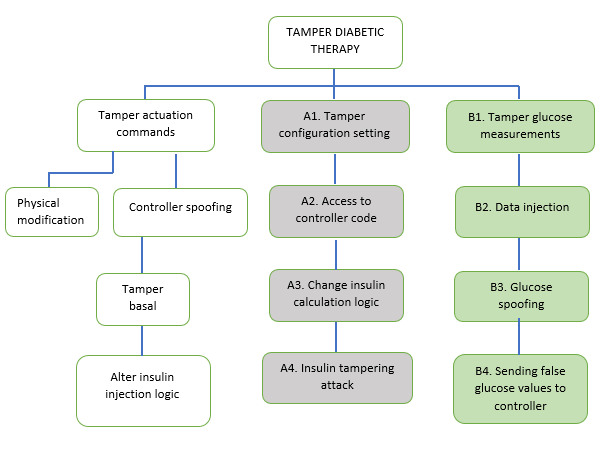
\includegraphics[scale=0.75,keepaspectratio = true]{Graphics/AttackTreeSAPNew.png}
    \caption{Attack tree for SAP}
    \label{fig:attackTreeOpenAPS}
\end{figure}

\begin{itemize}
\item {\bf Insulin Tampering Attack (Block A1-A4)}: Similar to battery tampering attack on an \ac{UAV}, insulin tampering attack also occurs when the attacker hacks the controller unit of the system i.e., \ac{OpenAPS}~\cite{radcliffe2011hacking}. After hacking, the attacker can modify the logic where the rate of insulin is calculated, based on the input blood glucose values sampled from the patient. This will lead to injection of faulty insulin dosage into the patients body which can prove fatal. Raspberry Pi 3 was used for our \ac{SAP} experiments and change in the control logic of the \ac{OpenAPS} was made to reflect this attack. After the attack had been planted, the insulin dosage command sent out by the controller was faulty as expected.

\item {\bf Glucose Spoofing Attack (Block B1-B4)}: The glucose spoofing attack modifies the value of the blood glucose contained in the data packets being sent from the patient. The incorrect value which will be substituted can be either greater than, or less than the measured blood glucose value. This change in the real value will lead the controller to calculate an incorrect value of insulin (though the logic through which insulin dose calculated is untouched), which will have harmful effects on the patient. This attack was mounted by injecting false data into the communication channel between the blood glucose monitor and the controller.
\end{itemize}

\section{Detection of attacks on \ac{SAP}}
\begin{itemize}
\item {\bf Insulin Tampering Attack}: As the attacker modifies only the insulin dosage while keeping the other properties the same, the intrusion detector is able to detect the attack, as the current correlation is not what it expects after its training phase. Similar to above attacks the log likelihood of the current system trace is less than that of the trained \ac{HMM}, thus arousing suspicion.
\item {\bf Glucose Spoofing Attack}:  The intrusion detector module of \ac{CORGIDS} receives the correlated properties which contains both faulty and non-faulty values of the blood glucose in it. Thus, based on this input data, the log likelihood generated by the current log differs from that expected by the trained \ac{HMM}. This indicates that there is an intrusion in the current state of the \ac{SAP}.
\end{itemize}

Although, the attacks that are demonstrated in this paper break the logical correlation directly, \ac{CORGIDS} is also capable of detecting an anomaly which is generated through indirect attacks. For example, instead of changing the physical property like battery \% left in the battery tampering attack (this is a attack in which correlations are broken directly), we could change either the value of some variable (other than the physical variable) used in the \ac{UAV} or alter other logic which does not directly effect the physical property (more details in ~\autoref{ch:comparisonwithrelatedwork}). These changes will propagate in the program and ultimately reach the receiving end of the \ac{CPS} (an actuator). If they do not, then the attack is likely to be harmless as the attacker cannot change the physical behavior of the \ac{CPS} without modifying its outputs. 

\endinput
=====================================================================
% EOF